\newchapstyle
\chapter{Collection of DC data of graphene Josephson devices}
%\chapter{Miscellaneous data on gJJs embedded in microwave circuits}
\label{chap:gJJmisc}

%\epigraph[0pt]{
%	Something.
%}{Someone}
%
%
\begin{abstract}
	\color{title}
	Here, we provide additional data of current-voltage curves of graphene Josephson junctions and SQUIDs embedded in DC bias microwave cavities.
\end{abstract}

%% Start the actual chapter on a new page.
\afterpage{\pagecolor{none}}\newpage

\section{JJ self-oscillations}
In the IV traces of all gJJ devices embedded in MW cavities, we found peculiar oscillations for bias currents exceeding $I_c$, in particular on the retrapping branch, as shown in Fig.~\ref{fig:IVoscillations}.
%
These oscillations occured without any MW probe tone applied, and seemed to be largely independent of gate voltage or magnetic field.
%
Upon closer inspection of the IV curves, we found that these oscillations stem from steps in the measured voltage, as shown in Fig.~\ref{fig:IVsteps}.

We attribute these to Fiske-like oscillations, due to the JJ probing its electromagnetic environment~\cite{fiskeTemperatureMagneticField1964,eckSelfDetectionAcJosephson1964,coonJosephsonAcStep1965}:
%
A voltage-biased Josephson junction is known to emit radiation according to the second Josephson relation,
%
\begin{align}
\frac{\partial \delta}{\partial t}=\frac{2e}{\hbar}V(t)
\end{align}
%
where $\delta$ is the phase across the junction.
%
This Josephson radiation can resonantly excite any present cavity modes with frequency $\omega_n=n2eV/\hbar$, $n\in\mathbb{Z}$.
%
In a current-voltage trace of a JJ, this results in steps at voltages
%
\begin{align}
V_n=\frac{\hbar}{2e}\omega_n=\frac{v_{ph}\pi}{L}n
\end{align}
%
with the phase velocity $v_{ph}$ and the cavity length $L$.

Fiske steps are usually known to occur as a result of standing electromagnetic waves in a cavity formed by the Josephson junction itself, and are hence prominent in large-area JJ~\cite{krasnovFiskeStepsIntrinsic1999,kimFiskeStepsStudied2005,yabukiSupercurrentVanWaals2016b,liHighQualityEpitaxialMgB2017}.
%
However in our devices, there is a patterned $\lambda/2$ MW cavity surrounding the gJJ which can form a pronounced cavity mode.


In Fig.~\ref{fig:IVsteps}, we show a subset of IVs that exhibit such voltage steps as a function of gate voltage and magnetic field, respectively.
%
Steps occur at integer multiples of approximately \SI{16.7}{\micro\volt}, which corresponds to a resonance frequency of \SI{8.1}{\giga\hertz}, deviating by about \SI{2}{\percent} from the expected resonance frequency $f_r\approx\SI{8.3}{\giga\hertz}$ our MW circuits are designed for (cf. Chapter~\ref{chap:gJJ-CPR}).
%
We note that specifically in the device shown here, we were unable to detect a cavity resonance when performing spectroscopy using a vector network analyzer due to large internal losses from residual normal metal around the JJ.
%
Nevertheless, the DC data shows the sensitivity of the JJ to its environment, even if internal losses are high.

\begin{figure}
	\centering
	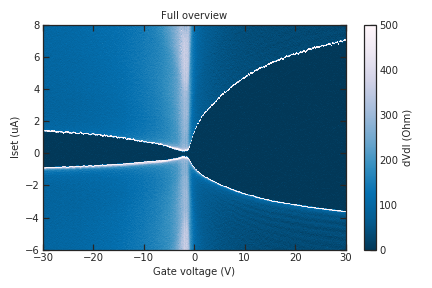
\includegraphics[width=0.45\linewidth]{chapter-gJJ-misc/figs/2x1}
	\hfill
	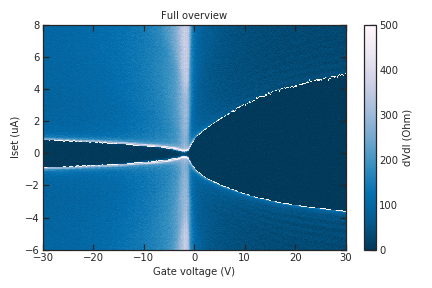
\includegraphics[width=0.45\linewidth]{chapter-gJJ-misc/figs/2x1_1K}
	\hfill
	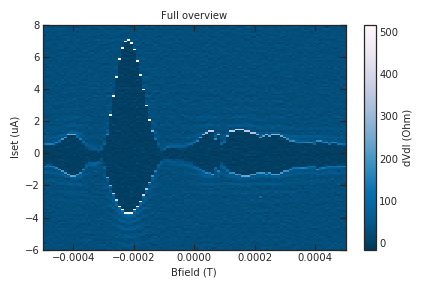
\includegraphics[width=0.45\linewidth]{chapter-gJJ-misc/figs/2x1_B}
	\hfill
	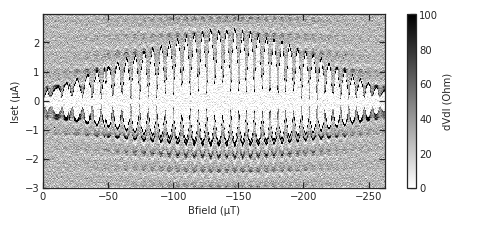
\includegraphics[width=0.45\linewidth]{chapter-gJJ-misc/figs/processing_DC_dVdI_2D_Bfield}
	\caption{IVoscillations}
	\label{fig:IVoscillations}
\end{figure}

\begin{figure}
	\centering
	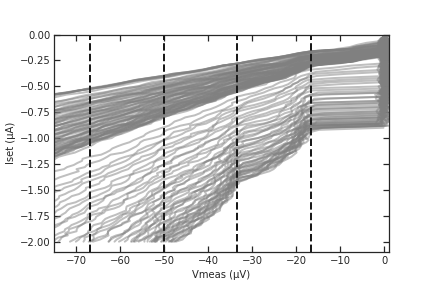
\includegraphics[width=0.45\linewidth]{chapter-gJJ-misc/figs/processing_DC_IsVm_Fiske_Vg}
	\hfill
	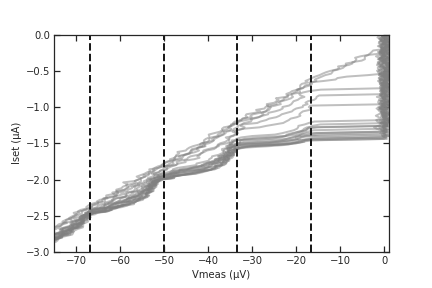
\includegraphics[width=0.45\linewidth]{chapter-gJJ-misc/figs/processing_DC_IsVm_Fiske_Bfield}
	\hfill
	\caption{IVsteps}
	\label{fig:IVsteps}
\end{figure}


\section{Shapiro steps}

In addition to voltage steps arising from self-oscillations of the JJ due to its electromagnetic environment, irradiating the JJ with microwaves can also lead to steps in the measured voltage, the so-called Shapiro steps~\cite{shapiroJosephsonCurrentsSuperconducting1963,kautzNoiseChaosJosephson1996,tinkhamIntroductionSuperconductivity1996,heerscheBipolarSupercurrentGraphene2007a,leeUltimatelyShortBallistic2015,shellyExistenceShapiroSteps2020,larsonZerobiasCrossingsPeculiar2020}.
%
We recorded several IV traces of graphene Josephson devices under MW radiation with varying frequency and power.
%
Here, we noted significant differences between power sweeps of a gJJ embedded in a low-loss MW cavity (Fig.~\ref{fig:Shapiro2x1}), and a gSQUID inside a MW cavity with high internal losses (Fig.~\ref{fig:ShapiroHero}).

\begin{figure}
	\centering
	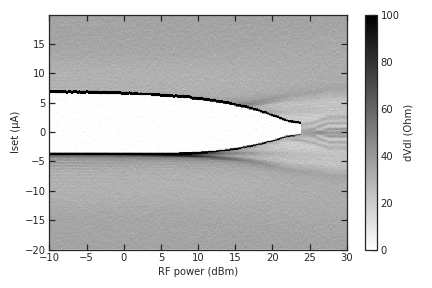
\includegraphics[width=0.45\linewidth]{chapter-gJJ-misc/figs/processing_Shapiro_2x1_5GHz}
	\hfill
	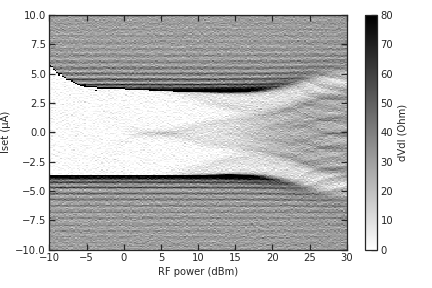
\includegraphics[width=0.45\linewidth]{chapter-gJJ-misc/figs/processing_Shapiro_2x1_onres}
	\caption{Shapiro steps of a gJJ in a low-loss MW cavity at \SI{5}{\giga\hertz} (off-resonant) and at \SI{8.1}{\giga\hertz} (on-resonance).}
	\label{fig:Shapiro2x1}
\end{figure}

\begin{figure}
	\centering
	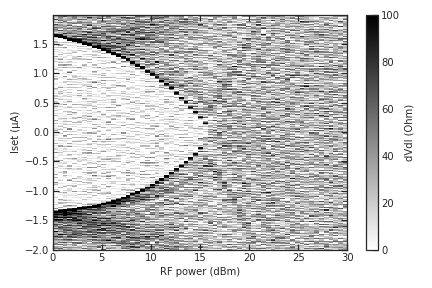
\includegraphics[width=0.3\linewidth]{chapter-gJJ-misc/figs/processing_Shapiro_Hero_3GHz}
	\hfill
	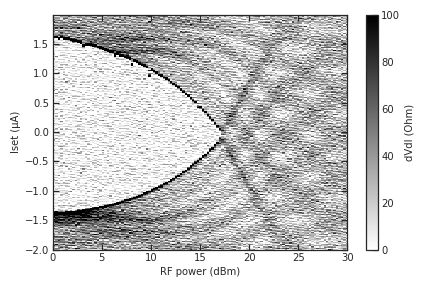
\includegraphics[width=0.3\linewidth]{chapter-gJJ-misc/figs/processing_Shapiro_Hero_5GHz_2}
	\hfill
	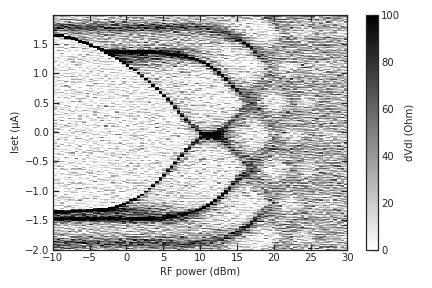
\includegraphics[width=0.3\linewidth]{chapter-gJJ-misc/figs/processing_Shapiro_Hero_8GHz_2}
	\caption{Shapiro steps of a gSQUID in a high-loss MW cavity at \SI{3}{\giga\hertz}, \SI{5}{\giga\hertz} and \SI{8}{\giga\hertz}..}
	\label{fig:ShapiroHero}
\end{figure}

Shapiro steps of the gSQUID as a function of drive frequency are shown in Fig.~\ref{Fig:Shapirofreq}.
%
Clearly, the voltage steps occur at multiple integer heights of $V=2e\omega/\hbar$.

\begin{figure}
	\centering
	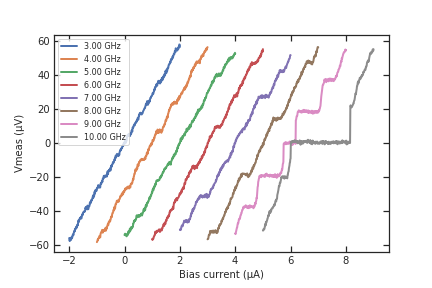
\includegraphics[width=0.45\linewidth]{chapter-gJJ-misc/figs/processing_Shapiro_Hero_freq_linecuts}
	\hfill
	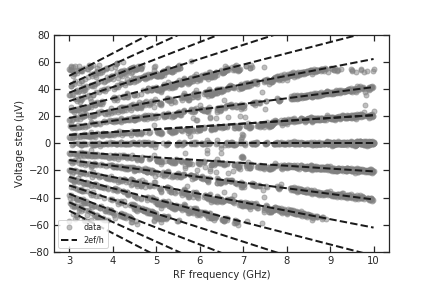
\includegraphics[width=0.45\linewidth]{chapter-gJJ-misc/figs/processing_Shapiro_Hero_freq_peaks}
	\hfill
	\caption{Shapiro steps of a gSQUID in a high-loss MW cavity at varying drive frequency.}
	\label{fig:Shapirofreq}
\end{figure}

%\clearpage
%\references{dissertation}

